\section{Tratamento Numérico}

\begin{frame}
    \frametitle{Abordagem}
    \begin{enumerate}
        \item Utilizamos o método \textit{Runge-Kutta} para a \textbf{discretização} e \textbf{resolução do sistema de equações diferenciais};
        \item Empregamos \textit{splines cúbicas} para a \textbf{representação gráfica};
        \item Aplicamos o \textit{Método dos Mínimos Quadrados (MMQ)} para a \textbf{análise da sensibilidade} do sistema.
    \end{enumerate}
        
        

\end{frame}

%------------------------------------------------

\begin{frame}
    \frametitle{Razões para a seleção do Método Runge-Kutta}
    Optamos pelo Método de Runge-Kutta pelos seguinte motivos:
    \begin{enumerate}
        \item O método escolhido calcula inclinações em quatro pontos dentro de cada intervalo de tempo, oferecendo uma aproximação mais precisa em comparação aos métodos aprendidos em aula.

        \item O método de quarta ordem possui um erro de truncamento local da ordem de $h^5$ e um erro de truncamento global da ordem de $h^4$, onde $h$ é o passo de tempo.
    \end{enumerate}
\end{frame}

%------------------------------------------------
\begin{frame}
    \frametitle{Método Runge-Kutta}

    Para as nossas simulações, os valores dos parâmetros utilizados são:

    \begin{block}{Parâmetros do sistema}
        \centering
        $\sigma = 10, \quad \rho = 28, \quad \beta = 8/3$
    \end{block}

    \begin{block}{Condições iniciais}
        \centering
        $x_0 = 0, \quad y_0 = 1, \quad z_0 = 1.05$
    \end{block}

    \begin{block}{Configurações do método}
        \centering
        Passo de tempo: $h = 0.01, \quad \text{Número de passos} = 1 \times 10^4$
    \end{block}

\end{frame}



%------------------------------------------------

\begin{frame}
    \frametitle{Evolução do atrator em função do número de passos}
    \begin{figure}[htbp]
        \centering
        \begin{minipage}{0.32\textwidth}
            \centering
            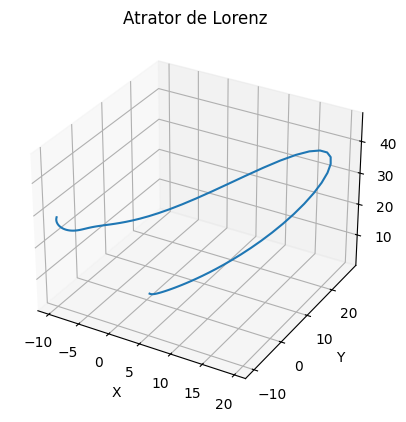
\includegraphics[width=\linewidth]{relatorio/img/attrator100.png}
            \vspace{0.5em} % Espaço para ajuste visual
            {\scriptsize $1 \times 10^2$ passos}
        \end{minipage}\hfill
        \begin{minipage}{0.32\textwidth}
            \centering
            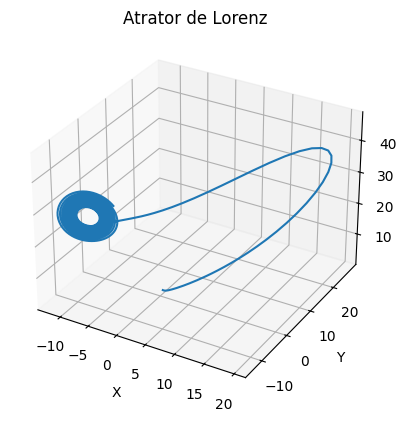
\includegraphics[width=\linewidth]{relatorio/img/attrator1000.png}
            \vspace{0.5em} % Espaço para ajuste visual
            {\scriptsize $1 \times 10^3$ passos}
        \end{minipage}\hfill
        \begin{minipage}{0.32\textwidth}
            \centering
            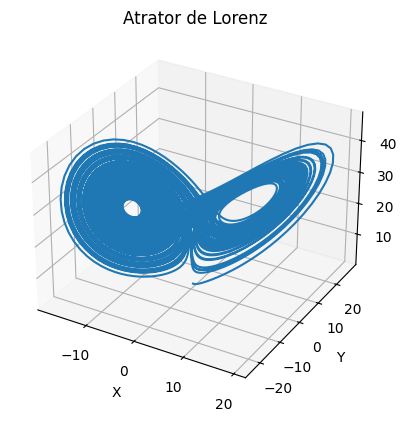
\includegraphics[width=\linewidth]{relatorio/img/attrator10000.png}
            \vspace{0.5em} % Espaço para ajuste visual
            {\scriptsize $1 \times 10^4$ passos}
        \end{minipage}
    \end{figure}
\end{frame}


%------------------------------------------------

\begin{frame}
    \frametitle{Justificativa do emprego de \textit{Spline} cúbicas}
    \begin{enumerate}
        \item Garantia de suavidade e continuidade nas curvas, essenciais dada a natureza não-linear e caótica do sistema. 
        \item Métodos, como o de Lagrange, não são adequados devido à perda de informação decorrente da linearização, comprometendo a representação precisa do sistema.
    \end{enumerate}
\end{frame}

%------------------------------------------------

\begin{frame}
    \frametitle{\textit{Spline} Cúbicas: resultado obtidos}      
    
    \begin{figure}
        \centering
        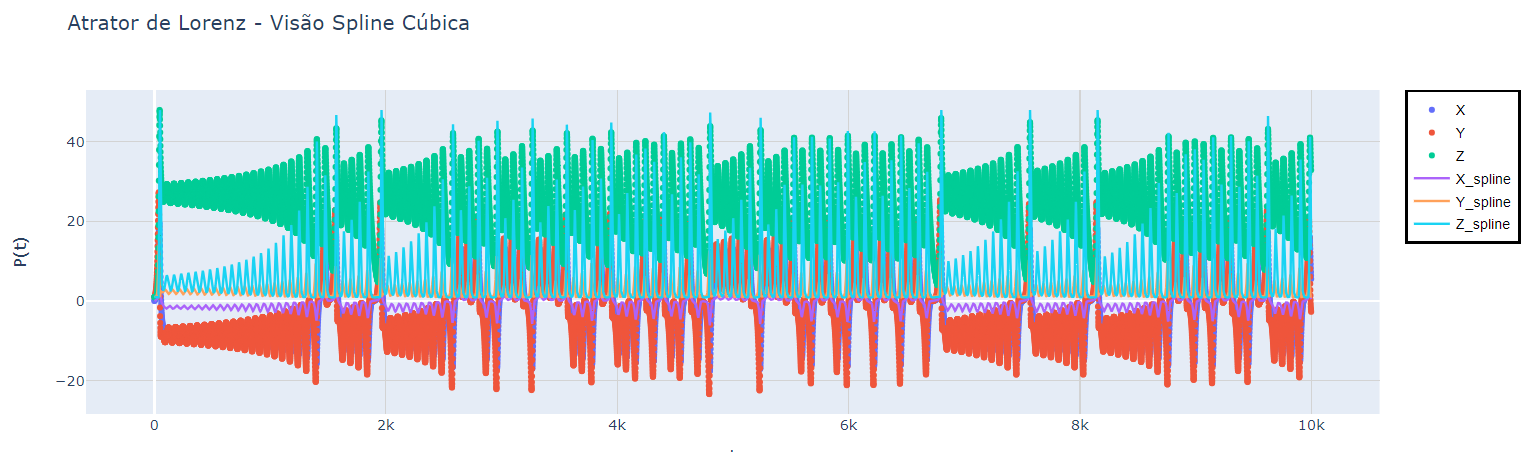
\includegraphics[width=1.0\textwidth]{relatorio/img/spline.png}
    \end{figure}

    \vspace{0.2cm}

    \begin{center}
        {\tiny Produzido pelos autores}
    \end{center}
    
\end{frame}
%------------------------------------------------

\begin{frame}
    \frametitle{Motivos para a adoção do MMQ}
    \begin{enumerate}
        \item O MMQ aproxima bem as dinâmicas não-lineares do sistema.
        \item Quantifica o impacto das alterações nos parâmetros e como pequenas mudanças afetam o sistema.
        \item Destaca-se pela alta eficiência computacional.
    \end{enumerate}
\end{frame}

%------------------------------------------------

\begin{frame}
    \frametitle{MMQ: Resultados obtidos}
    \begin{figure}
        \centering
        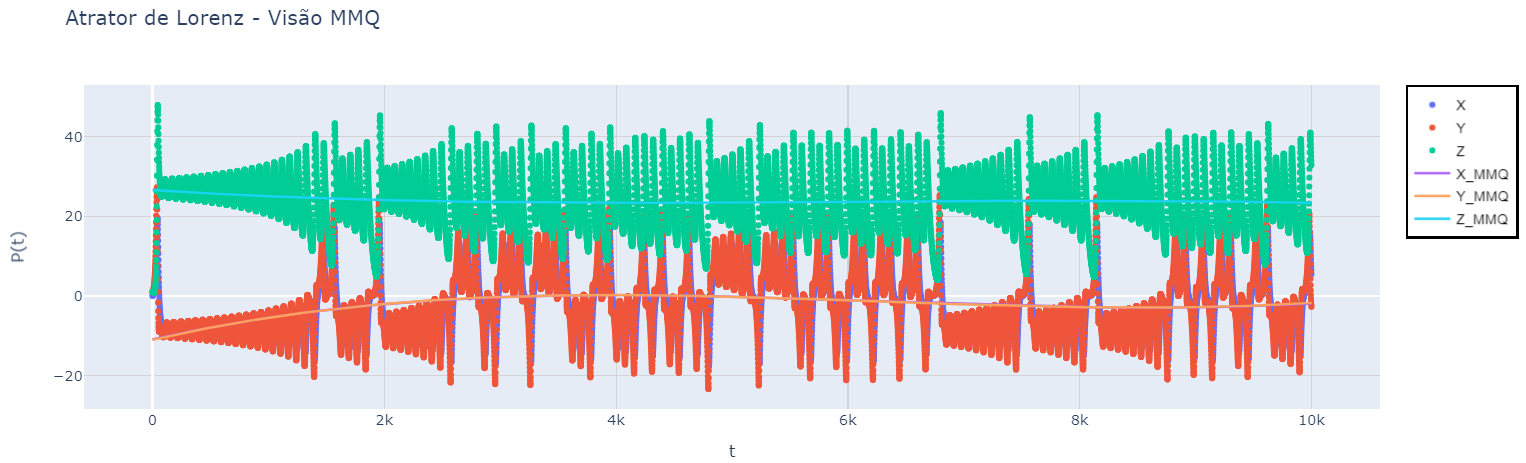
\includegraphics[width=1.0\textwidth]{relatorio/img/mmq.png}
    \end{figure}

    \vspace{0.2cm}

        \begin{center}
        {\tiny Produzido pelos autores}
    \end{center}
    
\end{frame}

